% Build with pdflatex pipeline.tex
\documentclass[tikz,border=6mm]{standalone}
\usepackage[T1]{fontenc}
\usepackage{lmodern}
\usetikzlibrary{arrows.meta,calc,fit,positioning}

\definecolor{ink}{HTML}{192D39}
\definecolor{blue}{HTML}{20547B}
\definecolor{pale}{HTML}{F1F6FA}
\definecolor{green}{HTML}{216554}
\definecolor{mint}{HTML}{EFF8F4}
\definecolor{amber}{HTML}{885314}
\definecolor{cream}{HTML}{FFF6E6}
\newcommand{\labeltext}[1]{{\bfseries\color{blue}#1}\par\smallskip}
\begin{document}
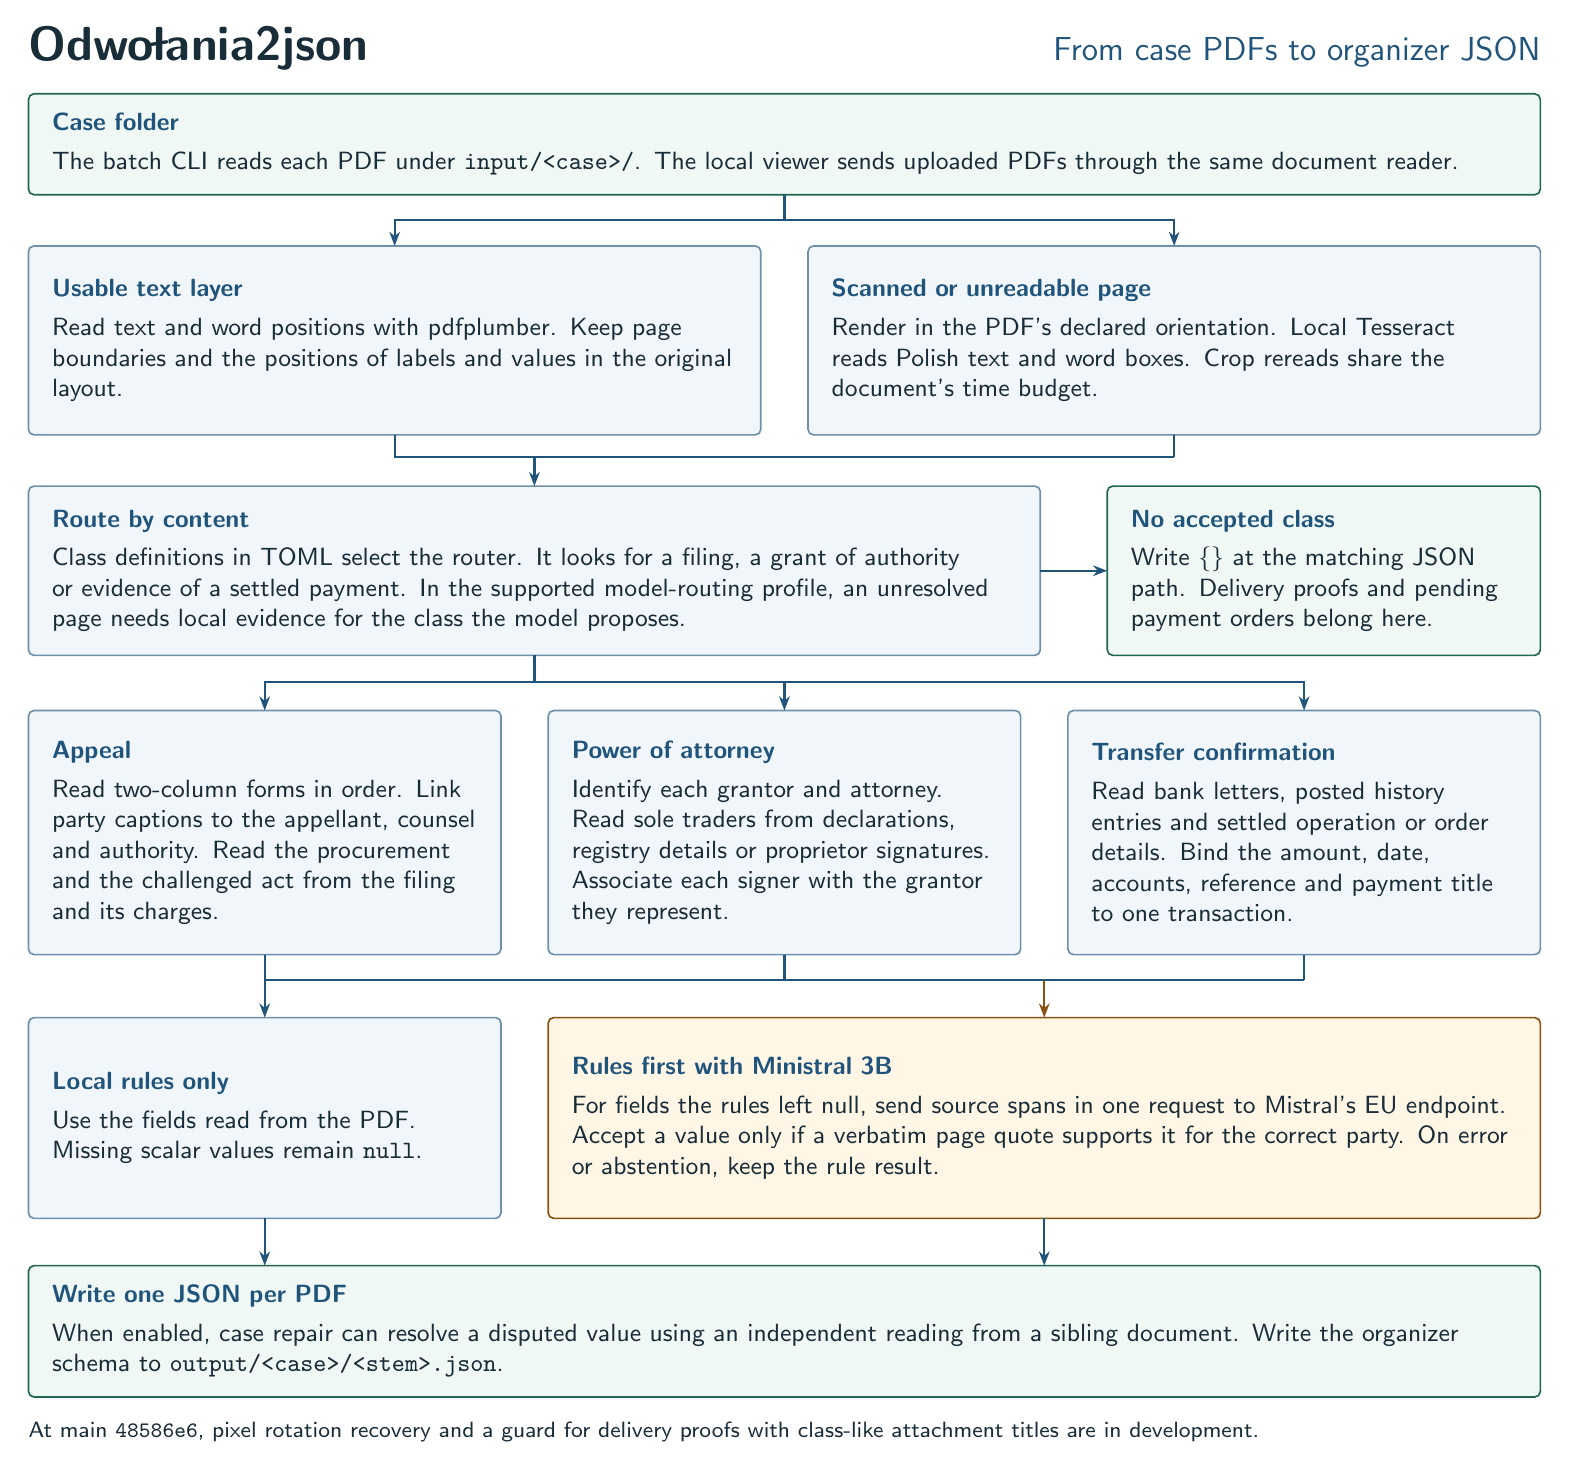
\begin{tikzpicture}[
    font=\sffamily\small, text=ink,
    card/.style={anchor=north west, align=left, text width=#1,
      inner xsep=3mm, inner ysep=2.5mm, rounded corners=2pt,
      draw=blue!65, fill=pale, line width=.6pt},
    terminal/.style={card=#1,draw=green,fill=mint},
    model/.style={card=#1,draw=amber,fill=cream},
    flow/.style={draw=blue,line width=.8pt},
    arrow/.style={flow,-{Stealth[length=1.8mm]}},
    endpoint/.style={draw=amber,line width=.8pt,-{Stealth[length=1.8mm]}},
    group/.style={inner sep=0pt,outer sep=0pt},
    every node/.append style={outer sep=0pt,execute at begin node={\hyphenpenalty=10000 }},
]
\node[anchor=south west,inner sep=0pt,font=\sffamily\bfseries\LARGE] at (0,.3)
  {Odwołania2json};
\node[anchor=south east,inner sep=0pt,font=\sffamily\large,text=blue] at (19.2,.34)
  {From case PDFs to organizer JSON};

\node[terminal=18.6cm] (input) at (0,0)
  {\labeltext{Case folder}The batch CLI reads each PDF under \texttt{input/<case>/}.
   The local viewer sends uploaded PDFs through the same document reader.};

\node[card=8.7cm,minimum height=2.4cm] (native) at ($(input.south west)+(0,-.65)$)
  {\labeltext{Usable text layer}Read text and word positions with pdfplumber.
   Keep page boundaries and the positions of labels and values in the original layout.};
\node[card=8.7cm,minimum height=2.4cm] (scan) at ($(native.north west)+(9.9,0)$)
  {\labeltext{Scanned or unreadable page}Render in the PDF's declared orientation.
   Local Tesseract reads Polish text and word boxes. Crop rereads share the document's time budget.};
\coordinate (readfork) at ($(input.south)+(0,-.32)$);
\draw[flow] (input.south) -- (readfork);
\foreach \r in {native,scan} \draw[arrow] (readfork) -| (\r.north);

\node[card=12.25cm,minimum height=2.15cm] (route) at ($(native.south west)+(0,-.65)$)
  {\labeltext{Route by content}Class definitions in TOML select the router. It looks for a filing, a grant of authority or
   evidence of a settled payment. In the supported model-routing profile, an unresolved
   page needs local evidence for the class the model proposes.};
\node[terminal=4.9cm,minimum height=2.15cm] (reject) at ($(route.north west)+(13.7,0)$)
  {\labeltext{No accepted class}Write \texttt{\{\}} at the matching JSON path.
   Delivery proofs and pending payment orders belong here.};
\coordinate (join) at ($(scan.south)+(0,-.28)$);
\draw[flow] (native.south) |- (join);
\draw[flow] (scan.south) -- (join);
\draw[arrow] (route.north |- join) -- (route.north);
\draw[arrow] (route.east) -- (reject.west);

\node[card=5.4cm,minimum height=3.1cm] (appeal) at ($(route.south west)+(0,-.7)$)
  {\labeltext{Appeal}Read two-column forms in order. Link party captions to the
   appellant, counsel and authority. Read the procurement and the challenged act
   from the filing and its charges.};
\node[card=5.4cm,minimum height=3.1cm] (grant) at ($(appeal.north west)+(6.6,0)$)
  {\labeltext{Power of attorney}Identify each grantor and attorney. Read sole traders
   from declarations, registry details or proprietor signatures. Associate each signer
   with the grantor they represent.};
\node[card=5.4cm,minimum height=3.1cm] (receipt) at ($(grant.north west)+(6.6,0)$)
  {\labeltext{Transfer confirmation}Read bank letters, posted history entries and
   settled operation or order details. Bind the amount, date, accounts, reference
   and payment title to one transaction.};
\coordinate (fork) at ($(route.south)+(0,-.34)$);
\draw[flow] (route.south) -- (fork);
\foreach \r in {appeal,grant,receipt} \draw[arrow] (fork) -| (\r.north);

\node[group,fit=(appeal)(grant)(receipt)] (readers) {};
\node[card=5.4cm,minimum height=2.55cm] (local) at ($(readers.south west)+(0,-.8)$)
  {\labeltext{Local rules only}Use the fields read from the PDF. Missing scalar values
   remain \texttt{null}.};
\node[model=12cm,minimum height=2.55cm] (keyed) at ($(local.north west)+(6.6,0)$)
  {\labeltext{Rules first with Ministral 3B}For fields the rules left null, send source spans in one request
   to Mistral's EU endpoint. Accept a value only if a verbatim page quote supports it
   for the correct party. On error or abstention, keep the rule result.};
\coordinate (bus) at ($(local.north)+(0,.48)$);
\foreach \r in {appeal,grant,receipt} \draw[flow] (\r.south) -- (\r.south |- bus);
\draw[flow] (appeal.south |- bus) -- (receipt.south |- bus);
\draw[arrow] (local.north |- bus) -- (local.north);
\draw[endpoint] (keyed.north |- bus) -- (keyed.north);

\node[terminal=18.6cm] (out) at ($(local.south west)+(0,-.6)$)
  {\labeltext{Write one JSON per PDF}When enabled, case repair can resolve a disputed value
   using an independent reading from a sibling document. Write the organizer schema to
   \texttt{output/<case>/<stem>.json}.};
\foreach \r in {local,keyed} \draw[arrow] (\r.south) -- (\r.south |- out.north);
\node[anchor=north west,align=left,text width=19.2cm,inner sep=0pt,font=\sffamily\footnotesize] at ($(out.south west)+(0,-.32)$)
  {At main \texttt{48586e6}, pixel rotation recovery and a guard for delivery proofs with class-like attachment titles are in development.};
\end{tikzpicture}
\end{document}
